\documentclass[a4paper, 11pt]{article}
\usepackage{geometry}
\geometry{letterpaper, margin=1in}
\usepackage{amsmath}
\usepackage{amssymb}  
\usepackage{amsthm}
\usepackage{ulem} 
\usepackage{graphicx}
\usepackage{hyperref} 
\graphicspath{ {images/} }

\begin{document}
%Header-Make sure you update this information!!!!
\noindent
\large\textbf{Optical Traps} \hfill \textbf{John Waczak} \\
\normalsize PH 431 \hfill  Date: \today \\
Prof. Bo Sun  \\


\section*{How Bessel beams generate forces} 
\paragraph{}
Previously, we derived that for the azimuthally symmetric solution to Maxwell's equations using Bessel's function we have a time averaged Poynting vector of the form: 
	\begin{equation}
		\langle S \rangle = I \propto J_1(k\sin(\alpha)\rho)^2
	\end{equation}
Where $\rho = \sqrt{x^2+y^2}$ is the cylindrical radius in the xy plane. This produces the familiar intensity cross section shown below which gives the beam it's special optical properties. 
	\begin{center}
		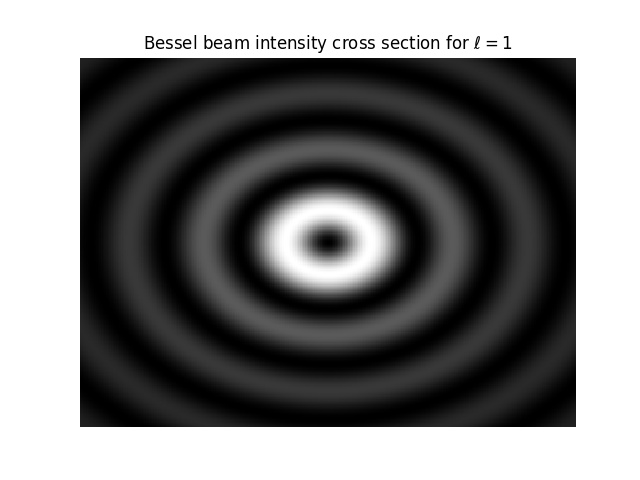
\includegraphics[scale=0.4]{intensityProfile}
	\end{center}
In the image, bright rings correspond to high intensity. Notice that for $\ell = 1$ beams we have a central dark spot. This is an important feature for optical traps as this is where the "trapped" particle rests. There are two distinct phenomena that enable these beams to generate forces on dielectric particles. They are gradient forces and radiation pressure. 

\subsection*{Gradient forces} 
\paragraph{}  
	According to the wave theory of light, the Bessel beam is a coupled system of oscillating electric and magnetic fields. Thus, when the beam encounters a dielectric material, it is possible for the electric field to induce a separation of charge allowing us to treat the object as a dipole $\mathbf{p}$ in an electric field $\mathbf{E}$. By Lorentz's law the force on such an object is given by the equation:
		\begin{equation}
			\mathbf{F} = \mathbf{p} \cdot \nabla\mathbf{E} 
		\end{equation}
	where $\nabla \mathbf{E}$ is evaluated by taking the gradient of the ith component of \textbf{E}. If we assume that the dipole is linearly polarized such that $\mathbf{p} = \epsilon\mathbf{E}$ (a reasonable assumption) then we can simplify the equation for \textbf{F} to: 
		\begin{eqnarray}
			\mathbf{F} = \frac{1}{2}\epsilon\nabla\mathbf{E}^2
		\end{eqnarray}
	Realistically, the fields oscillate so quickly that the measured force would be the time average $\langle \mathbf{F} \rangle$ of (3). For the Bessel beam we previously derived that the electric field has components in both the $\hat{\rho}$ and $\hat{z}$ directions therefore the gradient force points towards the location of greatest intensity (because we are taking the gradient). This can be accomplished by focusing the beam using lenses so that Bessel beam has a region of peak intensity as shown in the figure below: 
		\begin{center}
			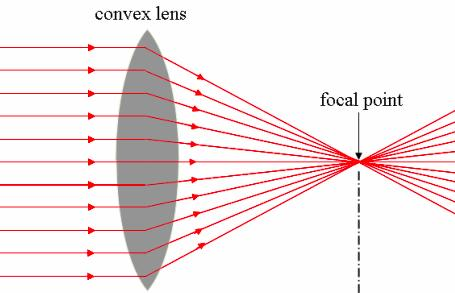
\includegraphics[scale=0.5]{focusedBeam}
		\end{center}
	
\subsection*{Radiation Pressure} 
	\paragraph{}
	According to Maxwell's equation, light can be treated as a transverse wave. It can be shown that these waves carry momentum and so due to the process of refraction, when a beam's path is diverted by the presence of a dielectric material, the beam's momentum is changed. The only way to resolve this is for the momentum of the object through which the beam travels to change in turn. This is visualized in the figure below: 
		\begin{center}
			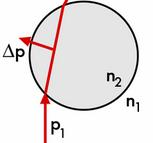
\includegraphics[scale=0.75]{sphereDiffraction}
		\end{center}
	
	\paragraph{}
	This image shows what would happen should the right side of the bead drift from the low intensity center into the high intensity ring. The beam's light would refract away from the center of the bead so that the net change in momentum of the bead would direct back towards the center of the beam. From this observed momentum change, we deduce that the beam is applying a force to the bead. This is why Bessel beams in particular are useful (as opposed to Gaussian profiles) because they persist over long distances i.e. non-diffracting so that the trap can be maintained throughout space.\\
	
\paragraph{}
Combining these two forces allows for the fine manipulation of particles in space. Controlling the polarization of Bessel beam tunes the size of the annuli. Combining this with a system of lenses to focus the beam allows for the 3-dimensional manipulation of dielectric particles. Furthermore, modern techniques take advantage of the superposition of multiple beams via holograms to enable the trapping of multiple particles in space. \\ 
	
	
	
\section*{Sources}  \url{http://home.uni-leipzig.de/pwm/web/?section=introduction&page=opticaltraps} 
	
	
	
	
	
	
	
	
	
	
	
	
	
	
	
	
	
	 
\end{document}